%% Comment this out if you'd rather use another style:
%\documentclass[preprint]{JASA}

%\documentclass[preprint,trackchanges]{JASA}

%\documentclass[preprint,NumberedRefs]{JASA}

% \documentclass[reprint]{JASA}

\documentclass[reprint,NumberedRefs]{JASA}

% \documentclass[reprint,TurnOnLineNumbers]{JASA}

\usepackage[caption=false]{subfig}

\begin{document}

\title[]{A novel multi-resolution method using wavelet packet transform and k-means clustering for analyzing data of passive cavitation detectors}

%% repeat as needed
\author{Max Au-Yeung}
\author{Reza Haqshenas}
%\author{Author Two}
%\author{Author Three}

\affiliation{Ultrasonics Laboratory, Department of Mechanical Engineering, University College London, London, UK}
\affiliation{Ultrasonics Laboratory, Department of Mechanical Engineering, University College London, London, UK}

\altaffiliation{}

%% for corresponding author
\email{zcemauy@ucl.ac.uk}

\begin{abstract}
Acoustic emissions from cavitating bubbles contain complex information in the time and frequency domains. Passive cavitation detectors are used to measure these emissions. By processing this data, it becomes possible to extract cavitation features including broadband emissions, harmonics, sub- and ultra-harmonics. This paper presents a novel approach that utilizes the wavelet packet transform, statistical metrics and k-means clustering to detect and classify these features in acoustic emissions. These findings enable us to quantitatively separate the stable and transient features of acoustic cavitation. This method was validated on acoustic emissions obtained by solving a single bubble dynamics (Gilmore-Akulichev model) and subsequently tested on experimental data from biomedical ultrasound applications.
\end{abstract}

\maketitle

%  End of title page for Preprint option --------------------------------- %

%% before appendix (optional) and bibliography:
\begin{acknowledgments}
This research was supported by ...
\end{acknowledgments}

\section{Introduction}
\label{sec:intro}

Acoustic cavitation refers to the formation, growth and oscillation of bubbles (cavities filled with gas and vapour) in a liquid using acoustic waves \cite{Leighton1994}. These bubbles may periodically oscillate whilst exposed to acoustic waves (known as stable cavitation) or grow and implode violently within a few cycles of excitation (known as inertial/transient cavitation). There are several physical effects associated with acoustic cavitation, including creation of free radicals, shock waves, shear stresses, micro-jets and micro-streaming in the insonated liquid \cite{Leighton1994}. To utilize these effects for different applications, ultrasound waves are widely used to produce acoustic cavitation, e.g. imaging ultrasound REF, therapeutic ultrasound REF, sono-chemistry, and sono-crystallization REF. To monitor these processes and to perform mechanistic studies, acoustic cavitation must be measured and evaluated quantitatively.

Passive REF and active REF cavitation detections are the two main techniques used to quantitatively measure acoustic emissions generated by bubbles. Passive techniques use a single element ultrasound transducer, i.e. passive cavitation detector (PCD), to acquire acoustic emissions whereas active techniques use more sophisticated ultrasound array transducers. Passive methods are cost-effective and easy to implement, hence they have been widely used in basic and applied research. Some examples in biomedical ultrasound are as follows: thermal ablation REF, histotripsy REF, drug and gene delivery REF, blood-brain-barrier opening REF. Several methods have been developed to analyze acoustic emissions from cavitations, including spectral techniques REFS, combination of spectral and digital filters REFS, time-frequency methods including short time-Fourier transform REF, Bilinear time-frequency distributions (Cohens Class distribution functions) REF, and wavelet transforms REF. These works detect and classify the two main types of acoustic cavitations qualitatively. To carry out fundamental studies and elucidate the concomitant biological/physical effects produced by acoustic cavitation, advanced signal processing techniques are required to detect, extract, classify and quantitatively characterize the features of acoustic cavitation. To tackle this problem, we present a new method which uses combined discrete wavelet packet transform and statistical signal processing for quantitatively analyzing acoustic emissions, extracting and classifying cavitation features. The method is implemented in a Python library which is available in a GitHub repository - see Section 2.2.

The method is discussed in detail in Section 2. For testing and verifying the efficacy of the method, synthetic acoustic emissions were generated by solving the problem of single bubble dynamics using Gilmore-Akulichev model, presented in Section 3. The method was then applied to analyze the theoretical acoustic emissions. Section 4 describes the experimental set up, procedure and data processing. 

\section{Materials and Methods}
\subsection{Features of acoustic cavitation}
The signal from a PCD contains multiple features: (i) a range of harmonics with frequency of $n f_0$ where $f_0$ is the fundamental frequency and $n=1,2,3,\dots$ is an integer. At low powers, the fundamental frequency is the only component \cite{neppiras1980acoustic}. As the ultrasound amplitude is increased, but before collapse cavitation occurs, high-order harmonics are emitted by the bubbles. The emission with frequency equal to twice fundamental was prominent and had an amplitude proportional to the square of the fundamental \cite{neppiras1980acoustic}. (ii) sub-harmonics with frequency of $f_0/n$. These components can be formed by both stable and inertial cavitation \cite{Leighton1994}. The main hypothesis about the formation of the sub-harmonics is that they are generated by the non-linear pulsations of stable cavitation. If they are emitted by a system with only inertial cavitation, this can be explained by the prolonged expansion phase that can occur when the bubble oscillates for a few cycles before collapsing. The 1/2 and 1/3 frequency sub-harmonics are the most commonly occurring ones in acoustic cavitation. (iii)ultra-harmonics with frequency of $mf_0/n$ where $m \neq n$ is an integer. These components can be formed by both stable and inertial cavitation \cite{Leighton1994}. (iv) broadband frequency component which is usually considered as an indicator of transient cavitation. The shock wave produced by an inertial collapse manifests as broadband noise in the spectrum \cite{frohly2000ultrasonic}. In the case of a cloud of bubbles, the interaction between bubbles can produce harmonics and sub- and ultra-harmonics as well \cite{yasui2010numerical}, further increasing the difficulty in analyzing the PCD data. 

These features have different types of time-frequency structures. The (sub- and ultra-) harmonic components of the signal exist for a long time interval but they have localised frequency values equal to $mf_0/n$ for integer $m$ and $n$ values. The transient components, however, have an in impulsive structure in time and relatively broadband structure in the frequency domain. The noise component (mainly measurement noise) exists over a long period and manifests as a broadband distribution in the frequency domain.

\subsection{Wavelet packet transform}\label{sec:WPT}

Wavelet packet bases were developed to effectively decompose a piecewise smooth signal with a varying time-frequency structure. Orthonormal wavelet packet bases divide the frequency axis into separate intervals of various sizes, known as scales. 
 
In fast orthogonal discrete wavelet transform (DWT), a bank of conjugate mirror filters and downsampling (by a factor of 2) are used to decompose a signal $x[n]$ of length $N=2^{n_0}$ into a cascade of coarser approximations $a_j[n]$ and finer details $d_j[n]$ at a scale $j$ [REF]
 
\begin{align}  
\label{eq:dwt-decomp}
a_{j+1}[n] ~&=~ \sum_{m=0}^{M-1} h[m]a_j[m-2n]  \\
d_{j+1}[n] ~&=~ \sum_{m=0}^{M-1} g[m]a_j[m-2n]  
\end{align}

\noindent where $a_0[n] = x[n]$, $h[m]$ and $g[m]$ are the impulse responses of the filters corresponding to the scaling and wavelet bases functions and are related as follows

\begin{align}  
\label{eq:dwt-filters}
g[m]~=~(-1)^{1-m} h[1-m]
\end{align}

\noindent $g[m]$ and $h[m]$ can be viewed as transfer functions of low- and high-pass filters, respectively, with length $M$. Thus, approximations and details represent the amplitudes of low- and high- frequency components, respectively, of the decomposed signal. In Eq. \ref{eq:dwt-decomp}, the approximations ($a_j$) are only divided to low- and high-frequency components. Instead, we can iteratively split both approximation ($a_j$) and detail ($d_j$) at each scale, usually represented in a binary tree. This increases the computational complexity of discrete wavelet packet transform (DWPT) to $O(Nlog_2(N))$ compared to $O(N)$ for DWT.
\noindent Any node of the binary tree includes a packet of wavelet transformed component, i.e., the coefficients of filtered signal at a frequency subband, and is labeled by tuple $(j,k)$ where $j$ is the scale number (the depth of the node in the tree) and $k$ is the number of nodes that are on its left at the same scale (position of a node at a given depth). A schematic diagram of discrete wavelet packet transform using a bank of filters is shown in Fig. \ref{fig:dwpt_filter_bank}.  

\begin{figure}
  \begin{center}
    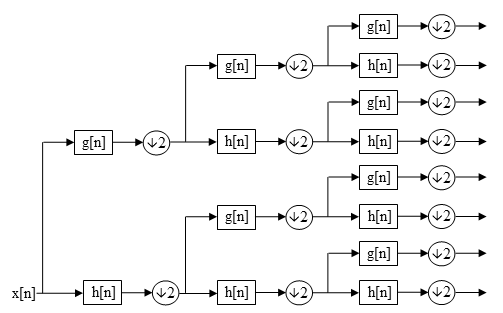
\includegraphics[width=3in]{./figs/dwpt_filter_bank}
  \end{center}
  \caption{The DWPT implemented as a filter bank}
  \label{fig:dwpt_filter_bank}
\end{figure}

Compared with discrete wavelet transform, DWPT provides higher frequency resolution (and decreased time resolution) at higher frequencies. The more levels of transform, the narrower the frequency subbands. We will use Shannon entropy minimization algorithm REF to find the maximum scales of decomposition for each signal.

The packets can be separately reconstructed into signals which combine to form the original signal. The stable and transient components of the signal tend to have different time-frequency signatures, so the transform will help separate them out. Once separated, the packets can be classified to give an indication of the presence and extent of each type of cavitation.


\subsection{Statistical metrics for feature detection}

To extract the signatures of inertial and stable cavitations at each subband, we will use the following statistical metrics: energy, kurtosis, crest factor, entropy and the logarithms of energy. These metrics are evaluated at the final (deepest) scale of DWPT. 

The energy of a packet is a measure of how much the signal is concentrated within that subband, calculated as follows

% \begin{align}
%   \label{eq:energy}
%   E_k^j = \dfrac{1}{N_k^j} {\mathbf{v}_k^j}^T \mathbf{v}_k^j 
% \end{align}

% \noindent where $\mathbf{v}_k^j$ is a vector containing the coefficients in a subband $(j,k)$ and $N_k^j$ is the number of coefficients in the subband.

\begin{align}
  \label{eq:energy}
  E_{j,k} = \sum_{n=1}^{N_{j,k}} x_{j,k}[n]^2 
\end{align}

\noindent where $x_{j,k}[n]$ are coefficients in a subband $(j,k)$ and $N_{j,k}$ is the number of coefficients in the subband. Note that using orthogonal wavelet bases for DWPT preserves the energy of the signal. Hence, the sum of the energy of all nodes in the final scale equals to the energy of the time series signal. To better distinguish fundamental, sub- and ultra-harmonics, we also use the log-energy metric, i.e., $LE_{j,k}~=~ \log{E_{j,k}}$. To measure the energy distribution of a subband - compared to other subbands, we use Shannon entropy which is defined as

\begin{align}
  \label{eq:entropy}
  S_{j,k} = -\sum_{n=1}^{N_{j,k}} \dfrac{x_{j,k}[n]^2}{E_{0,0}} ~ \log{\dfrac{x_{j,k}[n]^2}{E_{0,0}}} 
\end{align}

\noindent where $E_{0,0}$ is the total energy of the signal. The lower the entropy of a subband, the more deterministic components (information about harmonics) are within the subband. The transient components have a broadband frequency signature, hence a higher entropy can be attributed to transient and/or noise components of the signal. To distinguish these features we need additional statistical metrics.

Kurtosis is a measure of how often outliers occur in a signal. It is viewed as a metric for detecting transient cavitation. Kurtosis is calculated using the following relationship

\begin{align}
  \label{eq:kurtosis}
  K_{j,k} = \dfrac{1}{\sigma_{j,k}^4} \sum_{n=1}^{N_{j,k}}(x_{j,k}[n]-\overline{x}_{j,k})^4 
\end{align}

\noindent where $\overline{x}_{j,k}$ and $\sigma_{j,k}$ are the mean and standard deviation of the coefficients of the node $(j,k)$.

The crest factor is the ratio between the peak value and the mean of the signal, indicating how extreme the peaks are in the signal. It is obtained by

\begin{align}
  \label{eq:crest_factor}
  C_{j,k} = \dfrac{{\max{(\left\lvert x_{j,k}[n] \right\rvert )}}^2}{x_{rms}^2}
\end{align}
\noindent where $x_{rms}$ is the root-mean-square of $x_{j,k}[n]$.

A feature matrix of these statistical metrics of all subbands is formed. The next step of the algorithm is to classify these features, hence subbands. Different approaches are used for this end. A commonly used technique, adopted in our algorithm too, is k-means clustering \cite{yiakopoulos2011rolling, shete2013k}, which is discussed in the next section. 

\subsection{K-means clustering for feature classification}
After extracting features, the features can be classified using methods such as thresholding and clustering. K-means is a simple algorithm used for clustering. It groups the data into 'k' clusters. The aim of the algorithm is to minimise the total loss measured as the sum of the Euclidean distances between the centroid of the cluster and each point assigned to it (see equation \ref{eq:k-means}. To do this, the cluster centroids are initiated randomly and each data point is assigned to the nearest cluster. Next, the clusters are re-allocated to minimise the loss function. This process of shifting and reassigning the clusters are repeated until convergence.

\begin{align}
\Theta = \sum_{i=1}^{n}{\sum_{j=1}^{k}{\rho^{(i,j)} \lVert x^{(i)} - \mu^{(j)} \rVert^2}}
\label{eq:k-means}
\end{align}
Where Theta is the distortion (loss) function, $\rho$ is the assignment of the data point, $i$, to cluster, $j$, and $x$ and $\mu$ are the data point and cluster centroid respectively.

K-means is a non-convex optimisation problem and yields different results depending on the starting position of the clusters. There are several methods that have been developed to combat this, explained by Yiakopulos et al. \cite{yiakopoulos2011rolling}.

K-means has been combined with the wavelet transform in applications such as fault detection and EEG prediction. Both of these domains aim to categorise complex signals containing a mixture transients and harmonics. Yiakopulos et al. \cite{yiakopoulos2011rolling} applied the k-means algorithm to the problem of fault detection for rolling element bearings. Their method used two instances of K-means, one to determine whether the bearing was faulty and another to determine the nature of the fault. Each algorithm used a different set of used a different of features. They noticed that the non-convexity of k-means was a major disadvantage of the k-means algorithm and identified several techniques that have been developed to reduce the effect of this.  In their method, the centres were initialised using results from a dynamic model of the system. Shete et al. \cite{shete2013k} also used the k-means algorithm to detect the k-complex in EEG signals. This was achieved by using the k-means algorithm to compare feature of a reference k-complex signal and extracted sections of an input signal to determine whether that section contained a k-complex. This allows the training of the algorithm by providing it with examples of the feature that is sought after.

\subsection{Gilmore-Akulichev model}
One of them which agrees well with the most of experimental results on the oscillation of a spherical bubble \cite{lauterborn2010} and is valid for high Mach numbers is the Gilmore's model. Gilmore's model takes into account the compressibility of fluid and incorporates sound radiation from an oscillating bubble. The Gilmore equation is expressed as follows\cite{gilmore1952}:

\begin{align}
  \left(1~-~\dfrac{\dot{R}}{C}\right) R \ddot{R} ~+~ \dfrac{3}{2}\left(1~-~\dfrac{\dot{R}}{3C}\right){\dot{R}}^2 ~=~ \nonumber \\
  \left(1~+~\dfrac{\dot{R}}{C}\right) H ~+~ \dfrac{\dot{R}}{C}\left(1~-~\dfrac{\dot{R}}{C}\right) R \dfrac{d H}{d R}
\end{align}

\noindent where $C$ is the wave speed at the bubble's wall and $H$ is the enthalpy difference in the fluid at pressure $P$ and $P_\infty$. They are calculated using the following equations:
\begin{align}
\label{eq:Enthalpy}
H~=~\int_{P_\infty}^{P(R)} \dfrac{dP(\rho_L)}{\rho_L}
\end{align}
\begin{align}
	C ~=~ \sqrt{c^2~+~(n-1)H}
\end{align}

\noindent where $c$ is the wave speed at far-field. Gilmore used the Tait equation as the equation of state which reads:
\begin{align}
	\label{eq:State}
	P_L(\rho)~=~ A\left(\dfrac{\rho_L}{\rho_{L0}}\right)^n ~-~ B
\end{align}

\noindent substituting Equation \ref{eq:State} into Equation \ref{eq:Enthalpy}, enthalpy can be calculated as a function of the pressure as follows

\begin{align}
H ~=~ \dfrac{n A^{1/n}}{(n-1)\rho_L}  \left[ \left(P(R) ~+~ B\right)^{\left(1~-~1/n\right)} ~-~ \left(P_\infty ~+~ B\right)^{\left(1~-~1/n\right)} \right]
\end{align}

\noindent where $A, B,~\mathrm{and}~n$ are constants in the Tait equation which are obtained experimentally. In order to determine the enthalpy and the wave speed at the bubble's wall, it is required to calculate the value of pressure in the medium at the surface of the bubble, i.e., $P(R)$. This can be obtained using a modified Laplace equation as follows
\begin{align}
P(R)~=~ \left(P_0~+~\frac{2\sigma}{R_0}\right) \left(\dfrac{R_0}{R}\right)^{3\kappa}~-~\dfrac{2\sigma}{R}~-~\dfrac{4\mu \dot{R}}{R}
\end{align}

\noindent The Gilmore-Akulichev model was solved numerically for different sonication conditions. The implementation and numerical results were verified against published results for identical parameters.

\section{Results and discussion}

\subsection{Analyzing numerical results}

\subsection{Experimental set up and protocols}

\subsection{Analyzing experimental PCD data}
The signal from PCD is expected to contain a range of harmonics \cite{Leighton1994}. These have frequencies which are multiples of the fundamental frequency (the frequency of the ultrasound). Neppiras outlined the expected acoustic emissions for ultrasound at a range of power levels \cite{neppiras1980acoustic}. At low powers, the fundamental frequency was the only one measured. As the power was increased, but before collapse cavitation occurred, high-order harmonics were emitted by the bubbles. The emission with frequency equal to twice fundamental was prominent and had an amplitude proportional to the square of the fundamental.

Subharmonics occasionally appear. These have frequency of 1/N of the fundamental where N is an integer. This can be formed by both stable and inertial cavitation and there are many theories as to what may cause subharmonics \cite{Leighton1994}. The main theory is that they are generated by the non-linear pulsations of stable cavitation. If they are emitted by a system with only inertial cavitation, this can be explained by the prolonged expansion phase that can occur when the bubble oscillates for a few cycles before collapsing. The 1/2 and 1/3 frequency sub-harmonics are the most commonly occurring ones in acoustic cavitation.

The final component of the signal is broadband noise. There are several theories as to why this might occur. Most importantly, it is an indicator of transient cavitation. The shock wave is thought to cause this \cite{frohly2000ultrasonic}. Another possible cause for broadband noise is the bubble-to-bubble interaction, where bubbles pulsate non-periodically \cite{yasui2010numerical}. The interaction between bubbles is thought to produce harmonics and sub-harmonics as well, further increasing the difficulty in analysing clusters of bubbles. Broadband noise has the effect of increasing the intensity of each of the harmonics and sub-harmonics. The transducer will also produce some noise as well. The frequency ranges affected depends on the specifications of the transducer.
Overall, the feature extraction method must be able to separate and quantify harmonics, sub-harmonics, and broadband noise. This will make it possible to extract and classify features.


\subsubsection{Analysis}
The statistical measures give an indication of the strength and stablity of the signal in each frequency subband, allowing for the classification of stable and transient features. This is combined with thresholding, where the features are selected based on whether their statistical measures are above or below a given value. The illustrate the effect of thresholding, a synthetic signal (see figure \ref{fig:synth_signal} was transformed (see figure \ref{fig:dwpt_synth}). This data was generated using 2 sine waves with frequencies 1 and 100Hz. A series of short, high amplitude hanning windows were added to this to represent transients. Finally, the signal was windowed. No noise has been added.

The FFT of the signal represents the transients as a range of low amplitude frequencies as shown by the low level of background noise around the two peaks. In the wavelet packet transform, the transients are more visibly separated out across different subbands and more localised time. 

Next, the subbands are reconstructed to form waves reconstructed waves with the highest energy, kurtosis, and crest factor are shown in figure \ref{fig:highest_synth}. The highest energy subband was the lowest (fundamental) frequency. The second highest energy subband (not shown here) was the one containing the other frequency of 10Hz, indicating that energy will tend to pick out the high amplitude low frequency components. The subbands with the highest kurtosis were similar to the one shown in figure \ref{fig:highest_synth}. They were frequency subbands containing only transient components, indicating that kurtosis is a good measure of transience without any noise present. Finally, the subbands with the highest crest factor picked were those remaining in the lower frequency ranges. These contained some transient components mixed with the lower frequency sine waves.

When Gaussian noise is added to the data, the highest subbands sorted by energy and crest factor tends to remain the same, but the measure of kurtosis is impacted and will tend to return similar results to the crest factor.

\begin{figure}
\begin{center}
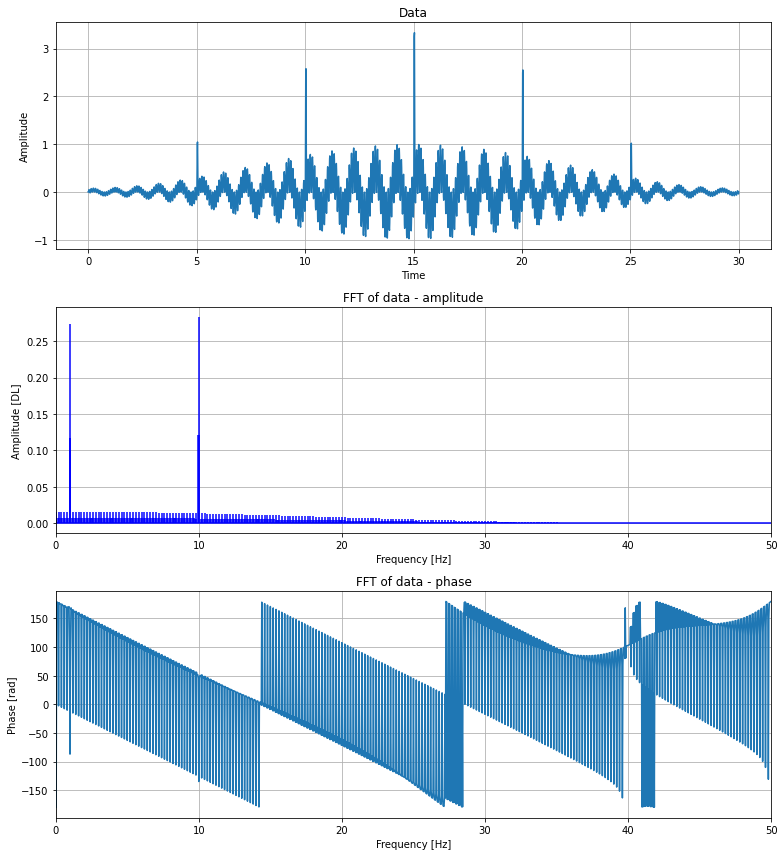
\includegraphics[width=3.5in]{./figs/synth_data}
\end{center}
\caption{synthetic data with sampling rate 100 with frequencies 1Hz and 10Hz, transient components, and noise.}
\label{fig:synth_signal}
\end{figure}

\begin{figure}
\begin{center}
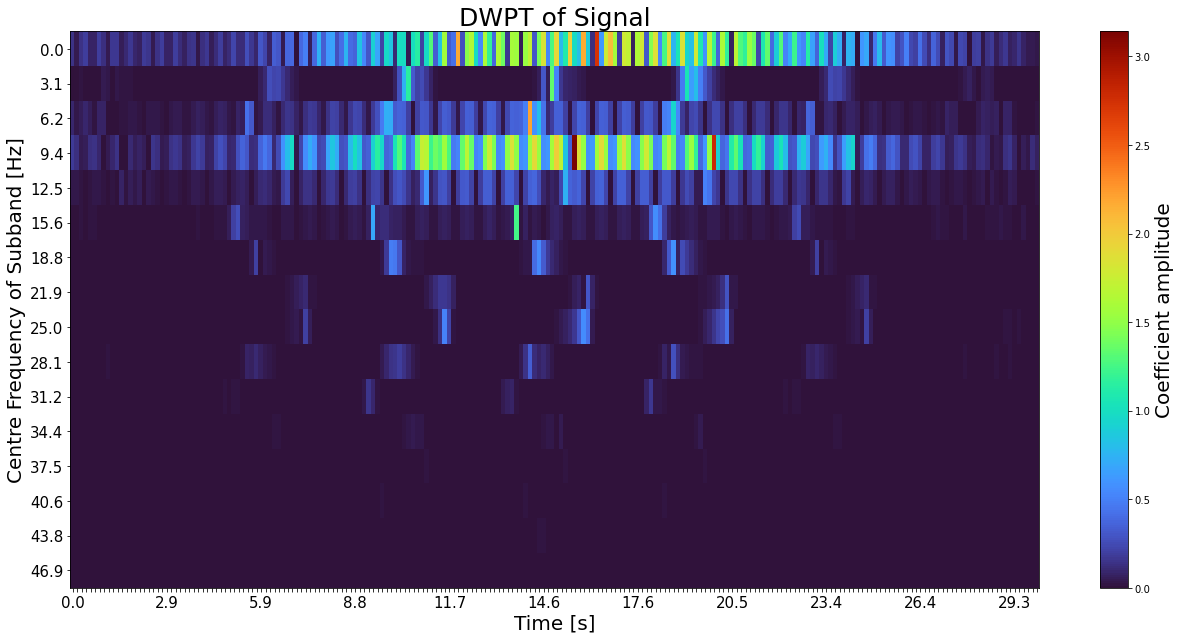
\includegraphics[width=3.5in]{./figs/dwpt_synth}
\end{center}
\caption{Heisenberg plot of a 4-level db16 DWPT of a synthetic signal in figure \ref{fig:synth_signal}.}
\label{fig:dwpt_synth}
\end{figure}

\begin{figure}
\begin{centering}
\subfloat[]{%
  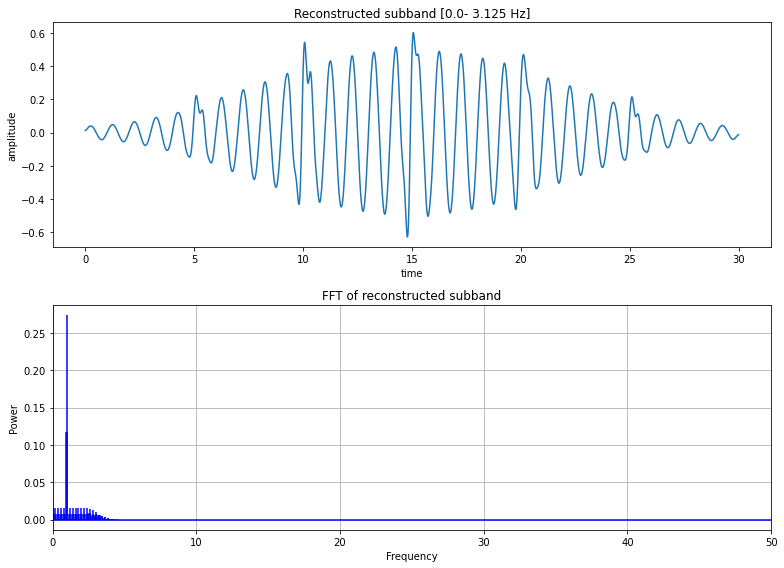
\includegraphics[clip,width=0.7\columnwidth]{./figs/highest_energy_synth}%
}
\hfill
\subfloat[]{%
  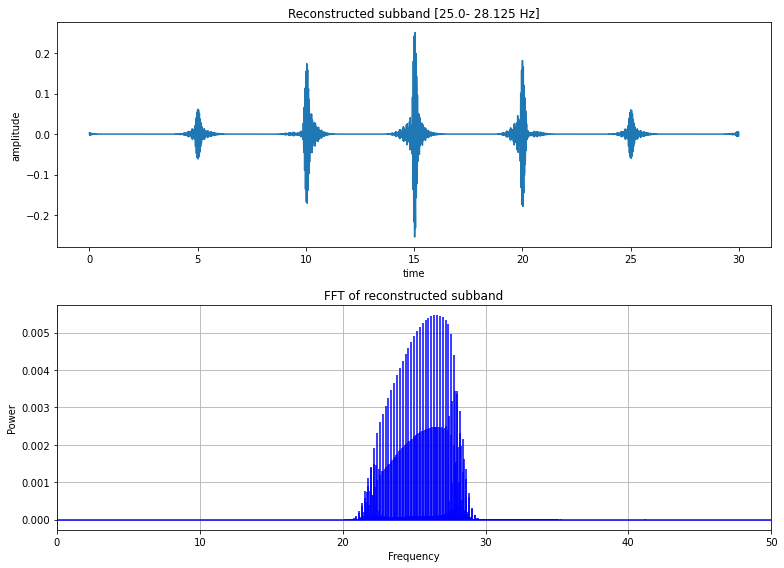
\includegraphics[clip,width=0.7\columnwidth]{./figs/highest_kurtosis_synth}%
}
\hfill
\subfloat[]{%
  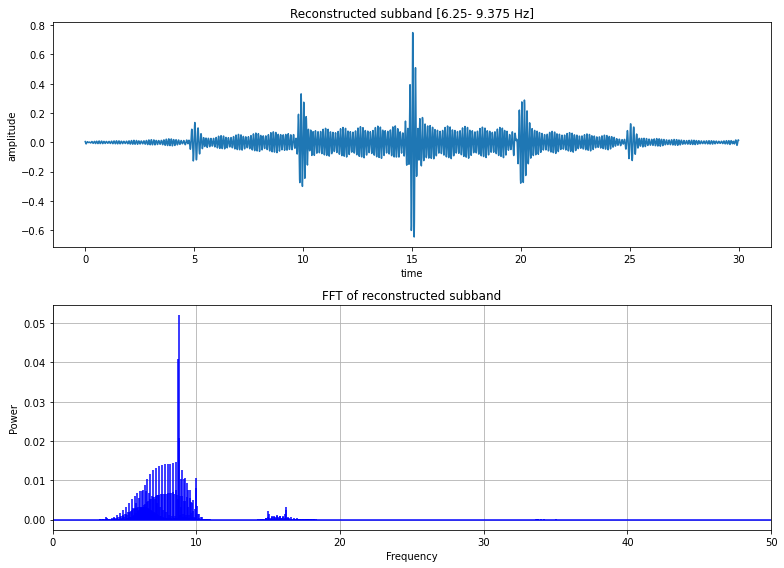
\includegraphics[clip,width=0.7\columnwidth]{./figs/highest_crest_synth}%
}
\hfill
\caption{Reconstructed subbands with highest energy (a), kurtosis (b), and crest factor (c) respectively}
\label{fig:highest_synth}
\end{centering}
\end{figure}

\section{Results}
\label{sec:results}

\section{Summary}
\label{sec:summary}
% ---------------------------------------------------------------------
% Appendix  (optional)

%\appendix
%\section{Appendix title}

%If only one appendix, please use
%\appendix*
%\section{Appendix title}

%% After first section in \appendix*,
%% \section{} the term APPENDIX will not be used.

%=======================================================
\section{References}
\bibliography{references}

%%When uploading your files to Editorial Manager,  include both the .bib and the appropriate .bst file (for author/year reference style: jasaauthoryear2.bst; for numerical style: jasanum2.bst). Both the .bib and .bst should be uploaded as the “Manuscript (TeX or Word only)” item type.


%=======================================================

\end{document}